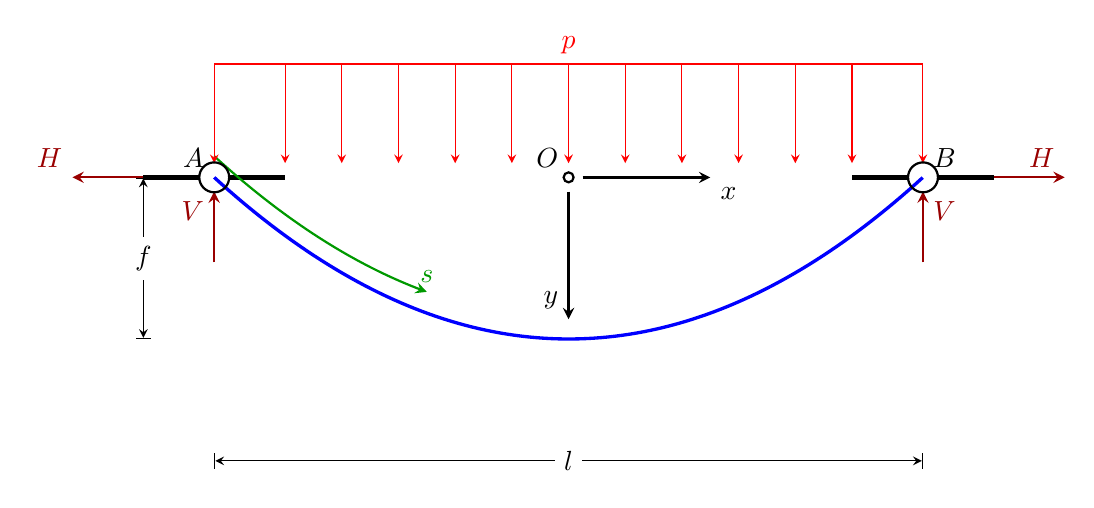
\begin{tikzpicture}[scale=1.8, >=stealth]
% Stile per i vincoli (muro/soffitto)
\tikzset{ground/.style={fill,pattern=north east lines,draw=none,minimum width=0.75cm,minimum height=0.3cm}}

% Parametri geometrici della parabola per il plot matematico
\def\l{5}   % Luce (lunghezza totale)
\def\f{1.14} % Freccia (distanza verticale dal vertice ad A/B: 3 - 1.86 = 1.14)

% Coordinate dei supporti
\coordinate (A) at (0,3);
\coordinate (B) at (5,3);
\coordinate (HA) at (-0.5,3);
\coordinate (HB) at (5.5,3);
\coordinate (VA) at (0,2.4);
\coordinate (VB) at (5,2.4);
\coordinate (O) at (2.5, 3);

% Rappresentazione dei supporti fisici
\draw[ultra thick] (-0.5,3) -- (-0.1,3);
\draw[ultra thick] ( 0.1,3) -- (0.5,3);
\draw[ultra thick] (4.5,3)  -- (4.9,3);
\draw[ultra thick] (5.1,3)  -- (5.5,3);

% --- LA FUNE (PARABOLA REALE) ---
% Equazione: y = 3 - f * (1 - (2*x/l - 1)^2)
\draw[very thick, blue, samples=100, domain=0:\l] 
    plot (\x, {3 - \f*(1 - (2*\x/\l-1)^2)});

% --- TRATTO DI ASCISSA CURVILINEA s (PARALLELA ALLA PARABOLA) ---
% Parte da A (x=0) e arriva fino a x=1.5, con un offset verticale di -0.15 per parallelismo
\draw[->, green!60!black, thick, samples=50, domain=0:1.5] 
    plot (\x, {3 - \f*(1 - (2*\x/\l-1)^2) + 0.15});

% Tratteggio verticale che collega la fine di 's' alla fune blue
\coordinate (S_end) at (1.5, {3 - \f*(1 - (2*1.5/\l-1)^2) + 0.15});
\coordinate (Fune_match) at (1.5, {3 - \f*(1 - (2*1.5/\l-1)^2)});

% Posizionamento MANUALE e preciso della lettera 's' sotto la punta della freccia verde
    \node[green!60!black, above] at (S_end) {$s$};

% --- CARICO DISTRIBUITO RETTANGOLARE SOPRA LA RETTA AB ---
\begin{scope}[shift={(A)}]
    \def\lung{5}      
    \def\alt{0.8}     
    
    \draw[red] (0, 0.1) -- (0, \alt) -- (\lung, \alt) -- (\lung, 0.1);
    
    \foreach \x in {0, 0.5, 0.9, 1.3, 1.7, 2.1, 2.5, 2.9, 3.3, 3.7, 4.1, 4.5, 5} {
        \draw[->, red, ] (\x, \alt) -- (\x, 0.1);
        }
    
    \node[red, above] at ({\lung/2}, \alt) {$p$};
\end{scope}

% --- QUOTE ---
\draw[black, thin, |<->|] (0, 1) -- (5, 1) node[midway, fill=white] {$l$};
\draw[black, thin, |<->|] (-0.5, 3) -- (-0.5, 1.86) node[midway, fill=white] {$f$};

% --- SISTEMA DI RIFERIMENTO ---
\draw[thick] (O) circle (1pt) node[above left] {$O$};
\draw[->, black, thick] (2.6, 3 ) -- (3.5, 3) node[below right]{${x}$};
\draw[->, black, thick] (2.5, 2.9 ) -- (2.5, 2) node[above left]{${y}$};

% Tensioni agli estremi
\draw[->, red!60!black, thick] (VA) -- ++( 0.0, 0.5) node[below left] {${V}$};
\draw[->, red!60!black, thick] (VB) -- ++( 0.0, 0.5) node[below right] {${V}$};
\draw[->, red!60!black, thick] (HA) -- ++(-0.5, 0.0) node[above left] {${H}$};
\draw[->, red!60!black, thick] (HB) -- ++( 0.5, 0.0) node[above left] {${H}$};

% Nodi di testo per i punti
\draw[thick] (A) circle (3pt) node[above left] {$A$};
\draw[thick] (B) circle (3pt) node[above right] {$B$};

\end{tikzpicture}